\section{Application}
In this section we will document the work done on the application during the first sprint.
The focus here was to implement functionality that gave a lot of value, and was easy to implement.

The following features were implemented:
\begin{itemize}
    \item Login screen
    \item Application selection screen
    \item Create application screen
    \item Create user screen
    \item Task dashboard screen
    \item Create task screen
\end{itemize}

Some of the functionality in this version of the application is mocked, because they are yet to be implemented on the backend.
This is however limited to task functionality, where the rest is actual data transmitted from the API.

\subsection{Design}
\label{sprint_1_design}
The screens were designed to give an idea of how the application should look.
The designs relevant to the features developed in this sprint can be seen on the following figures~\autoref{login_screen_design},~\autoref{app_selection_screen},~\autoref{create_task_screen} and~\autoref{task_dashboard_screen}.

The screens were designed to have a generic look and feel familiar to users.
The screens also follow the design standards set by Google in 'Design for Android' \cite{AndroidDesign}
The design process was done with all group members present and drawing on a whiteboard.



The tasks screen, which can be seen on~\autoref{task_dashboard_screen}, was designed to look like a kanban board.
A kanban board is an agile project management tool, designed to visualize work.
Kanban boards are often constructed of 3 columns each with their own status. In our case the status' are 'Not started', 'Work in progress' and 'Done' ordered from left to right.
The columns can be populated with tasks, which can be moved from left to right to indicate how along in the process they are.

This is done because Kanban boards are a common way to organise tasks, and is easy to understand, and has a very easy learning curve. \cite{kanbanBoard}

\begin{figure}[H]
    \centering
    \begin{minipage}{0.45\textwidth}
        \centering
        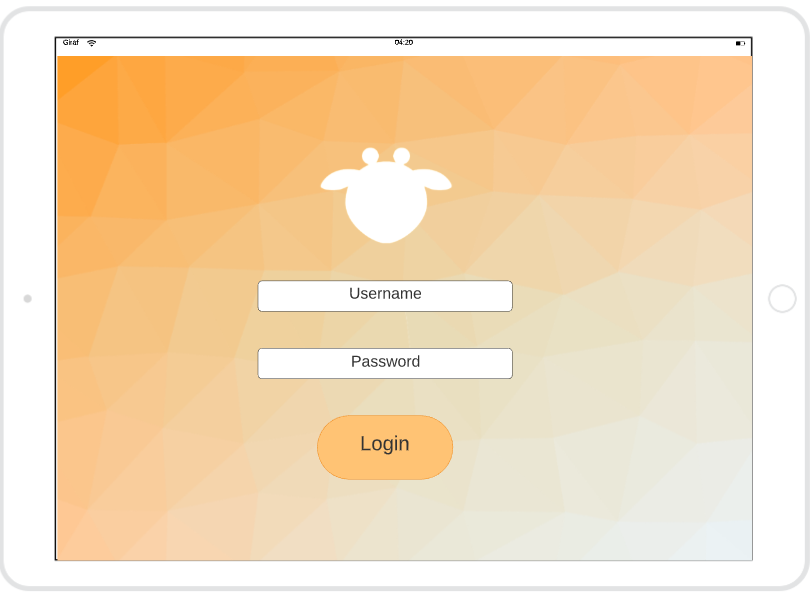
\includegraphics[width=0.9\textwidth]{Sprint_1/images/login_screen.png}
        \caption{Login screen design.}
        \label{login_screen_design}
    \end{minipage}\hfill
    \begin{minipage}{0.45\textwidth}
        \centering
        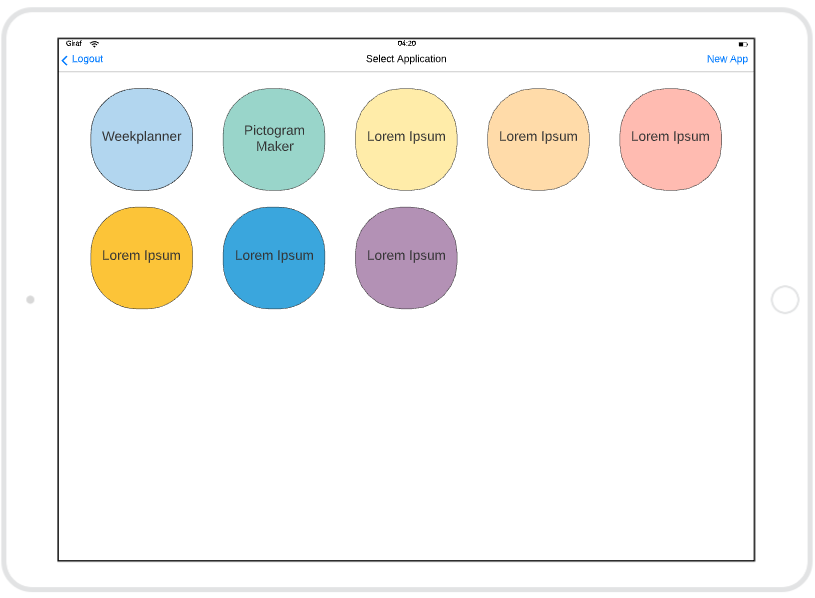
\includegraphics[width=0.9\textwidth]{Sprint_1/images/app_selection_screen.png}
        \caption{Application selection screen design.}
        \label{app_selection_screen}
    \end{minipage}
\end{figure}


\begin{figure}[H]
    \centering
    \begin{minipage}{0.45\textwidth}
        \centering
        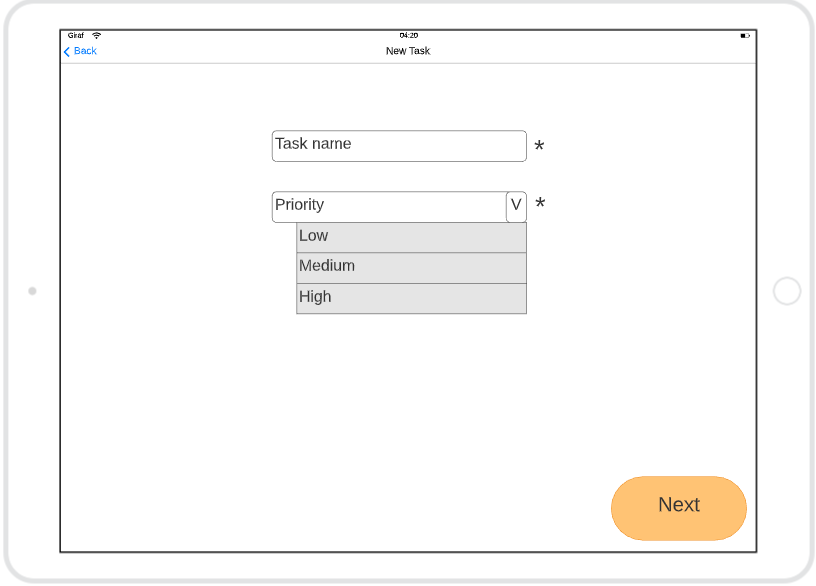
\includegraphics[width=0.9\textwidth]{Sprint_1/images/create_task_screen.png}
        \caption{Create task screen design.}
        \label{create_task_screen}
    \end{minipage}\hfill
    \begin{minipage}{0.45\textwidth}
        \centering
        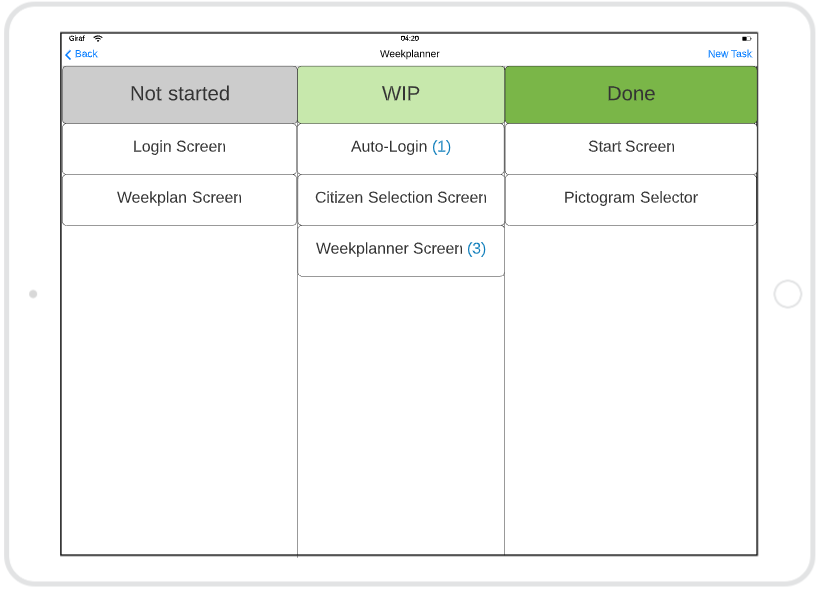
\includegraphics[width=0.9\textwidth]{Sprint_1/images/task_dashboard_screen.png}
        \caption{Task dashboard screen design.}
        \label{task_dashboard_screen}
    \end{minipage}
\end{figure}

\subsection{Implementation}
Most of this sprint was used on setting up the project and some code was written to allow for easier future development.
This includes a base screen that all other screens should extend, which adds nice-to-have functionality such as detecting if the device is a tablet or phone, and if it is in portrait or landscape mode.

The screens shown in~\autoref{sprint_1_design} have been implemented, and screenshots of the implementations can be seen in~\autoref{login_screen_design_app},~\autoref{app_selection_screen_app},~\autoref{app_creation_screen_app}, ~\autoref{create_task_screen_app} and~\autoref{task_dashboard_screen_app}.

The screens implemented have the needed functionality, but no tasks are shown in the Task screen~(~\autoref{task_dashboard_screen_app}), because this functionality was not yet implemented in the API.
But the application is ready for when this is implemented in Sprint 2.

The application code currently features all functionality available in the API as of Sprint 1.
However it is not all code that is used, but this makes it easy to implement new functionality without the need for implementing more API specific code. 


\begin{figure}[H]
    \centering
    \begin{minipage}{0.45\textwidth}
        \centering
        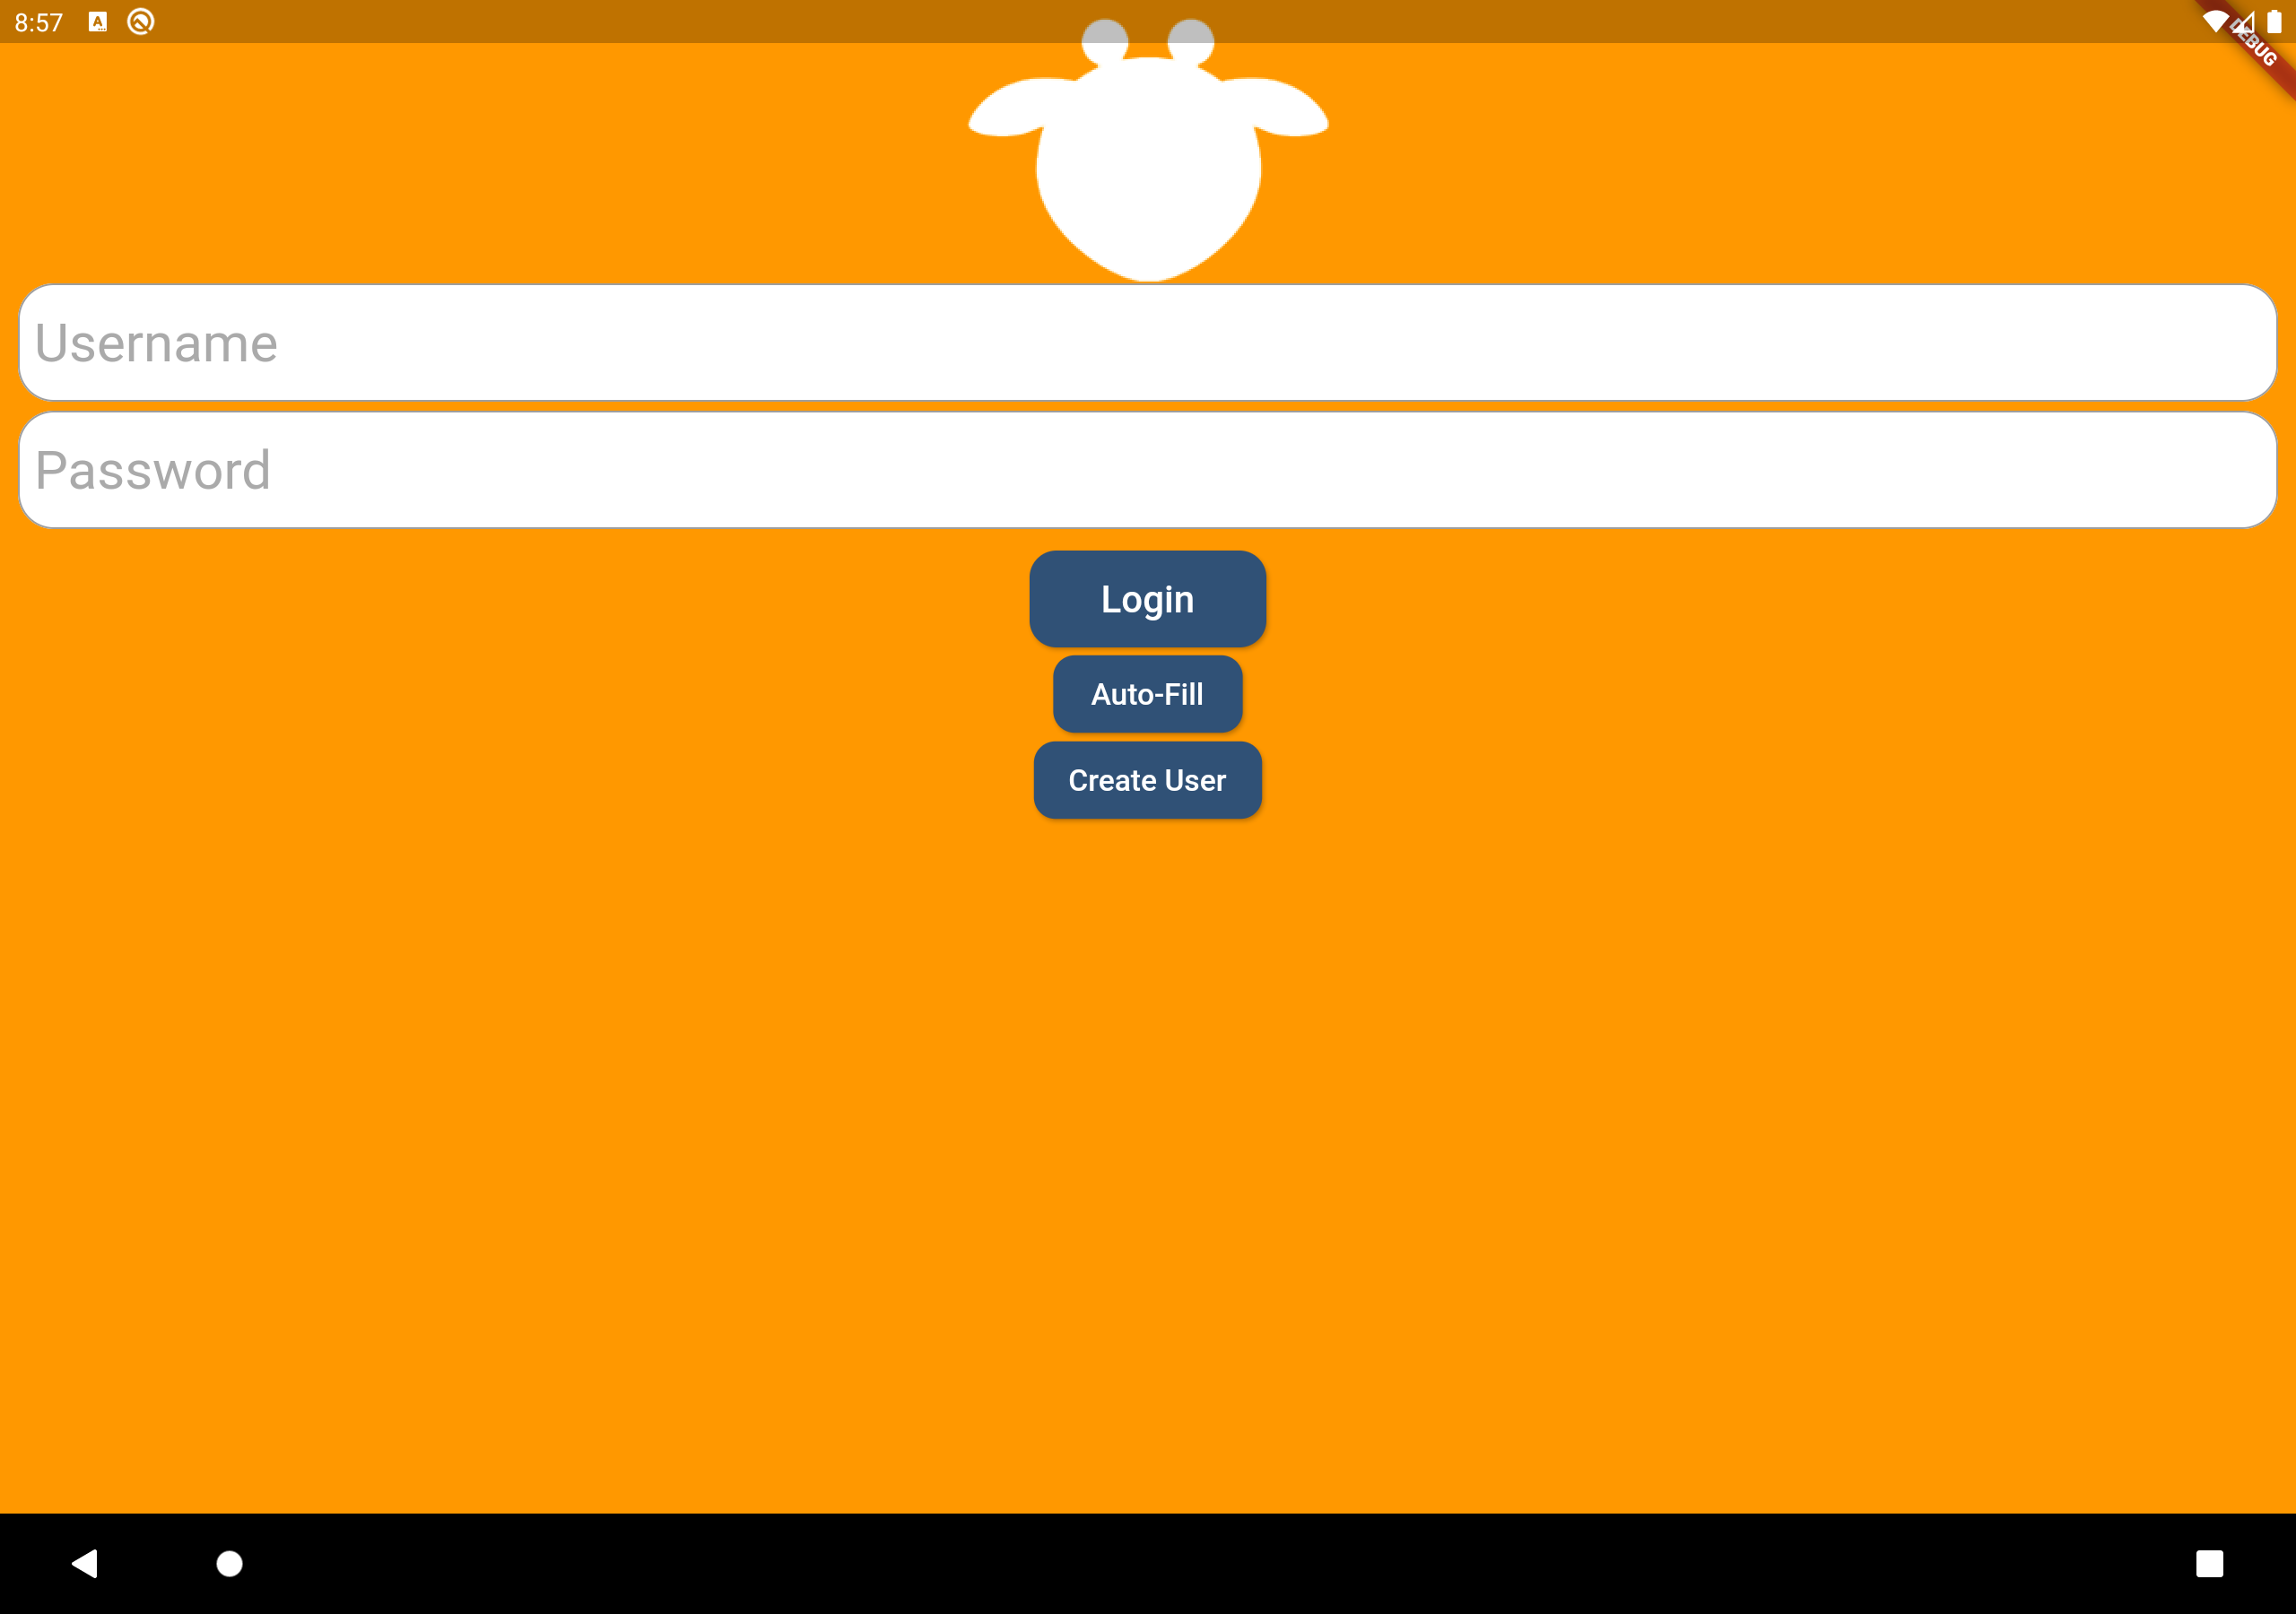
\includegraphics[width=0.9\textwidth]{Sprint_1/images/login_screen_app.png}
        \caption{Login screen implementation.}
        \label{login_screen_design_app}
    \end{minipage}\hfill
    \begin{minipage}{0.45\textwidth}
        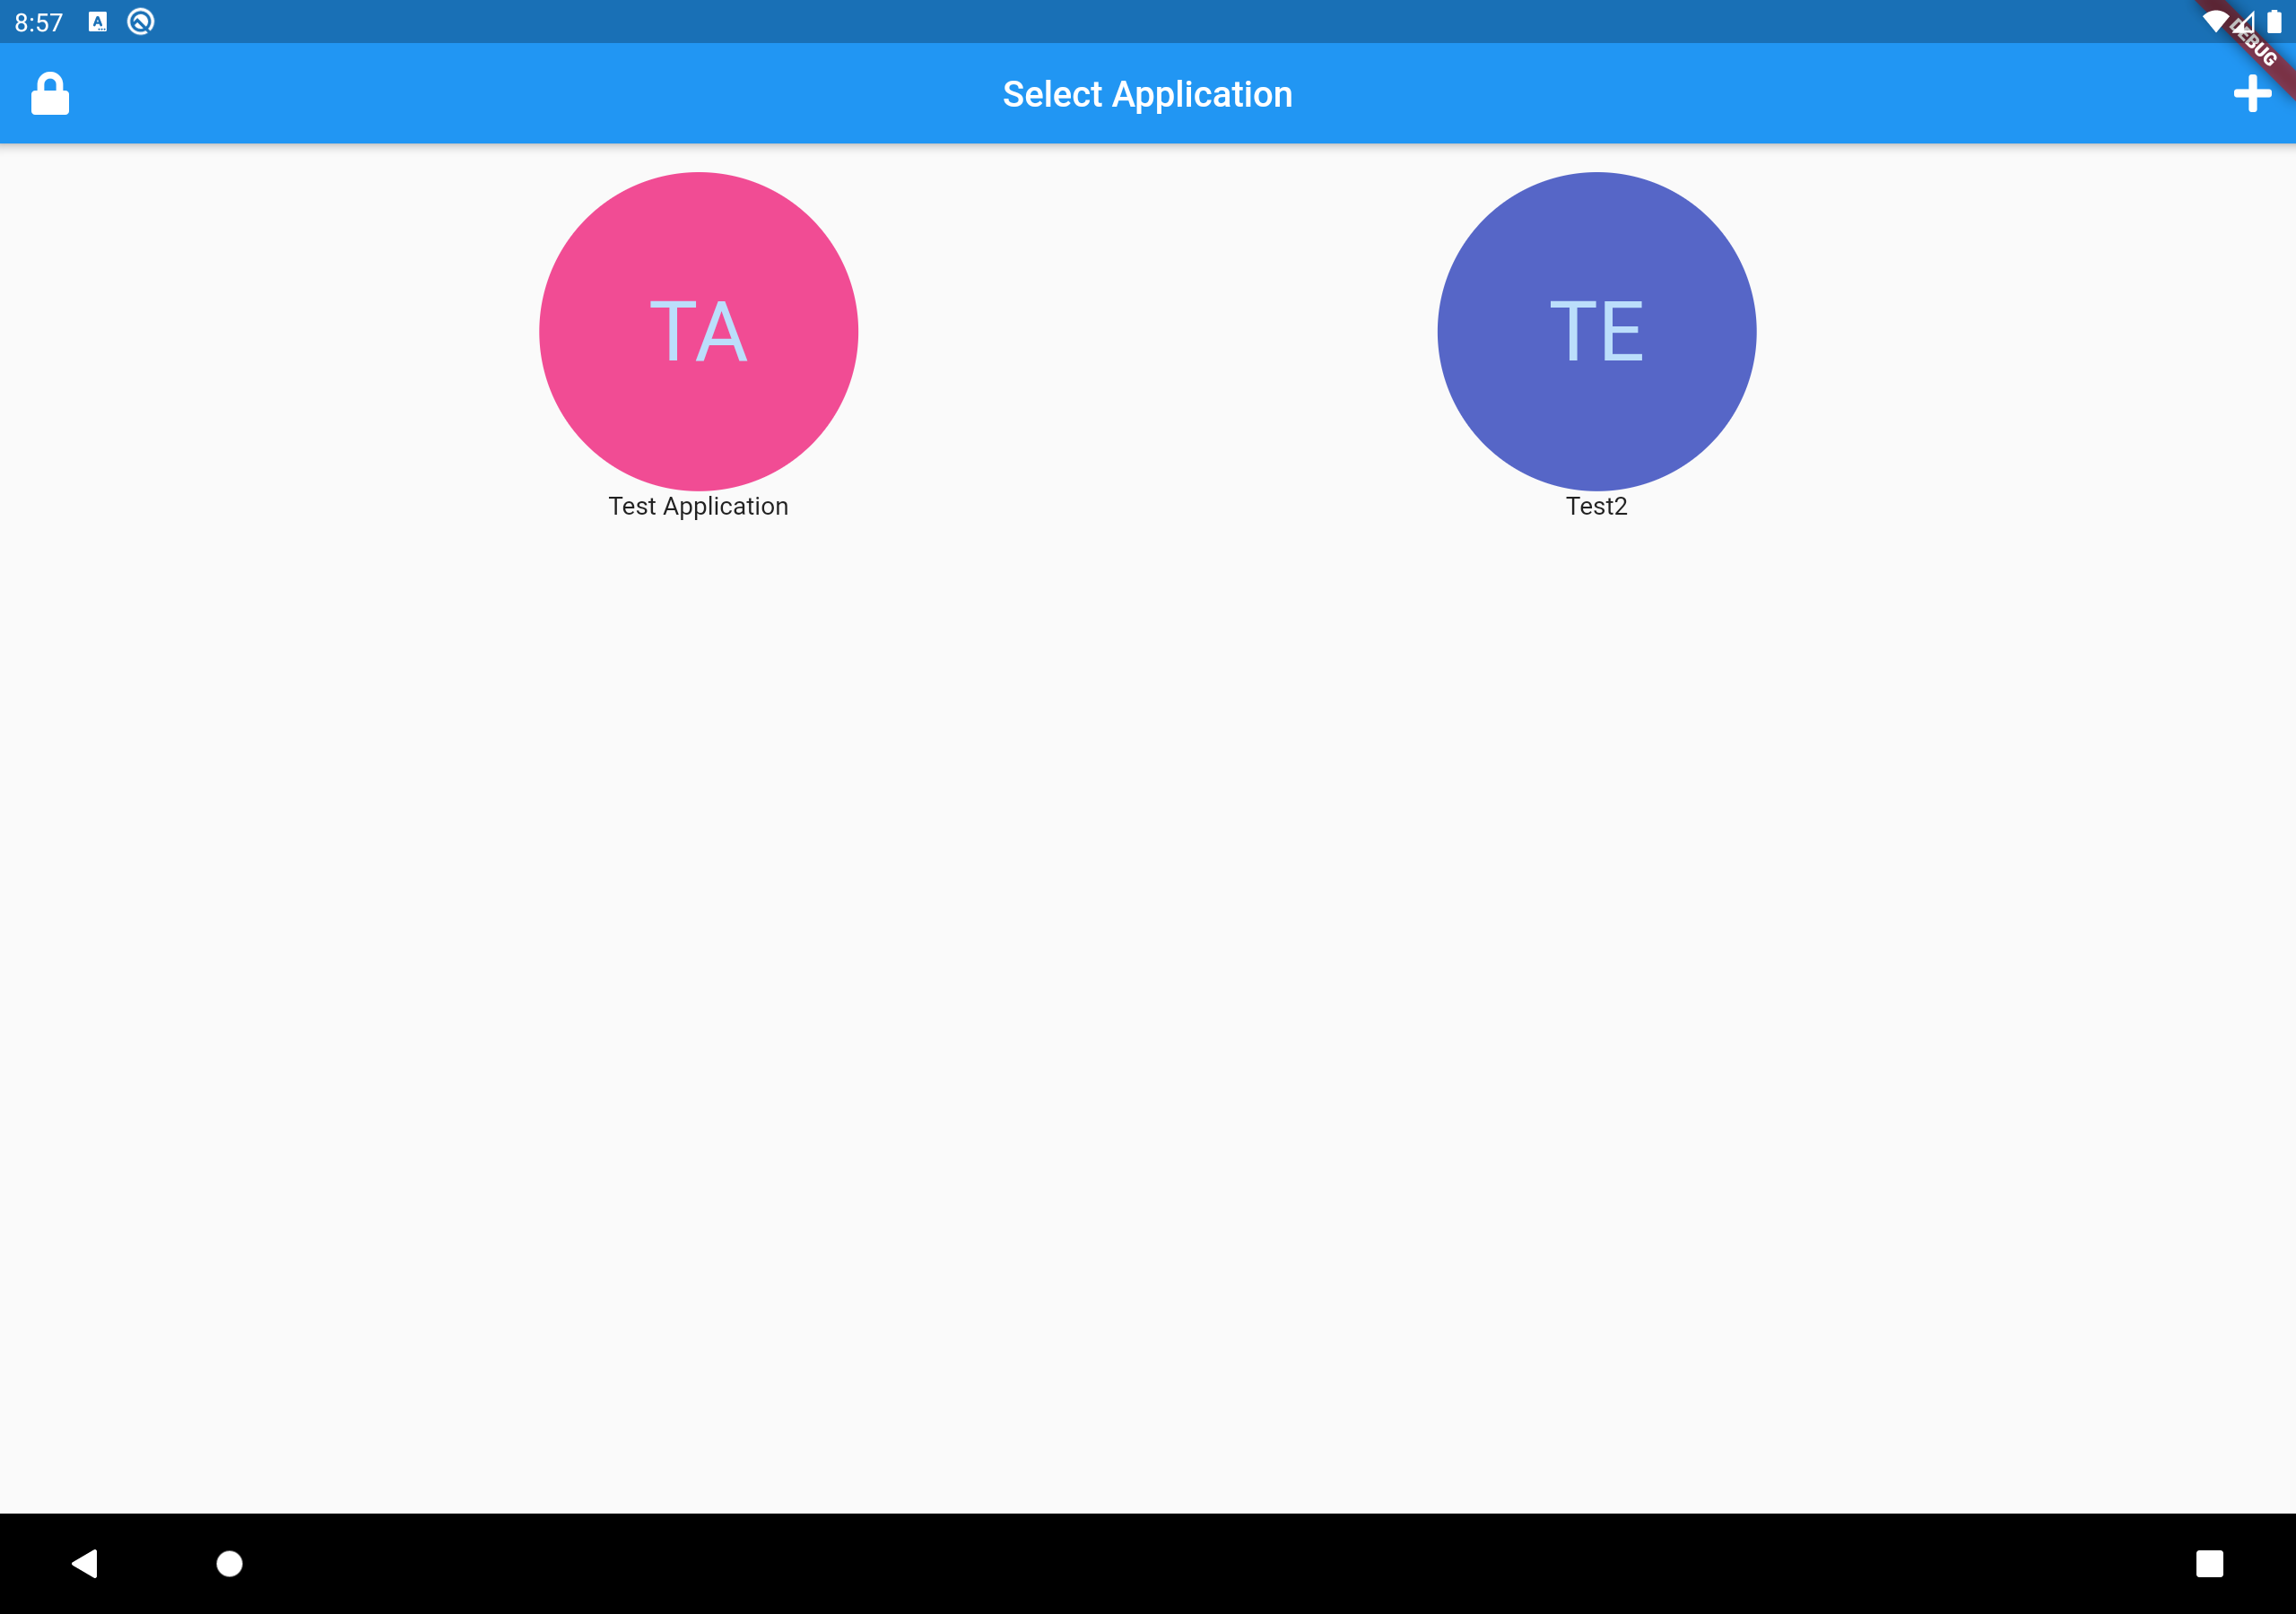
\includegraphics[width=0.9\textwidth]{Sprint_1/images/app_selection_screen_app.png}
        \caption{Application selection screen implementation.}
        \label{app_selection_screen_app}
    \end{minipage}
\end{figure}

\begin{figure}[H]
    \centering
    \begin{minipage}{0.45\textwidth}
        \centering
        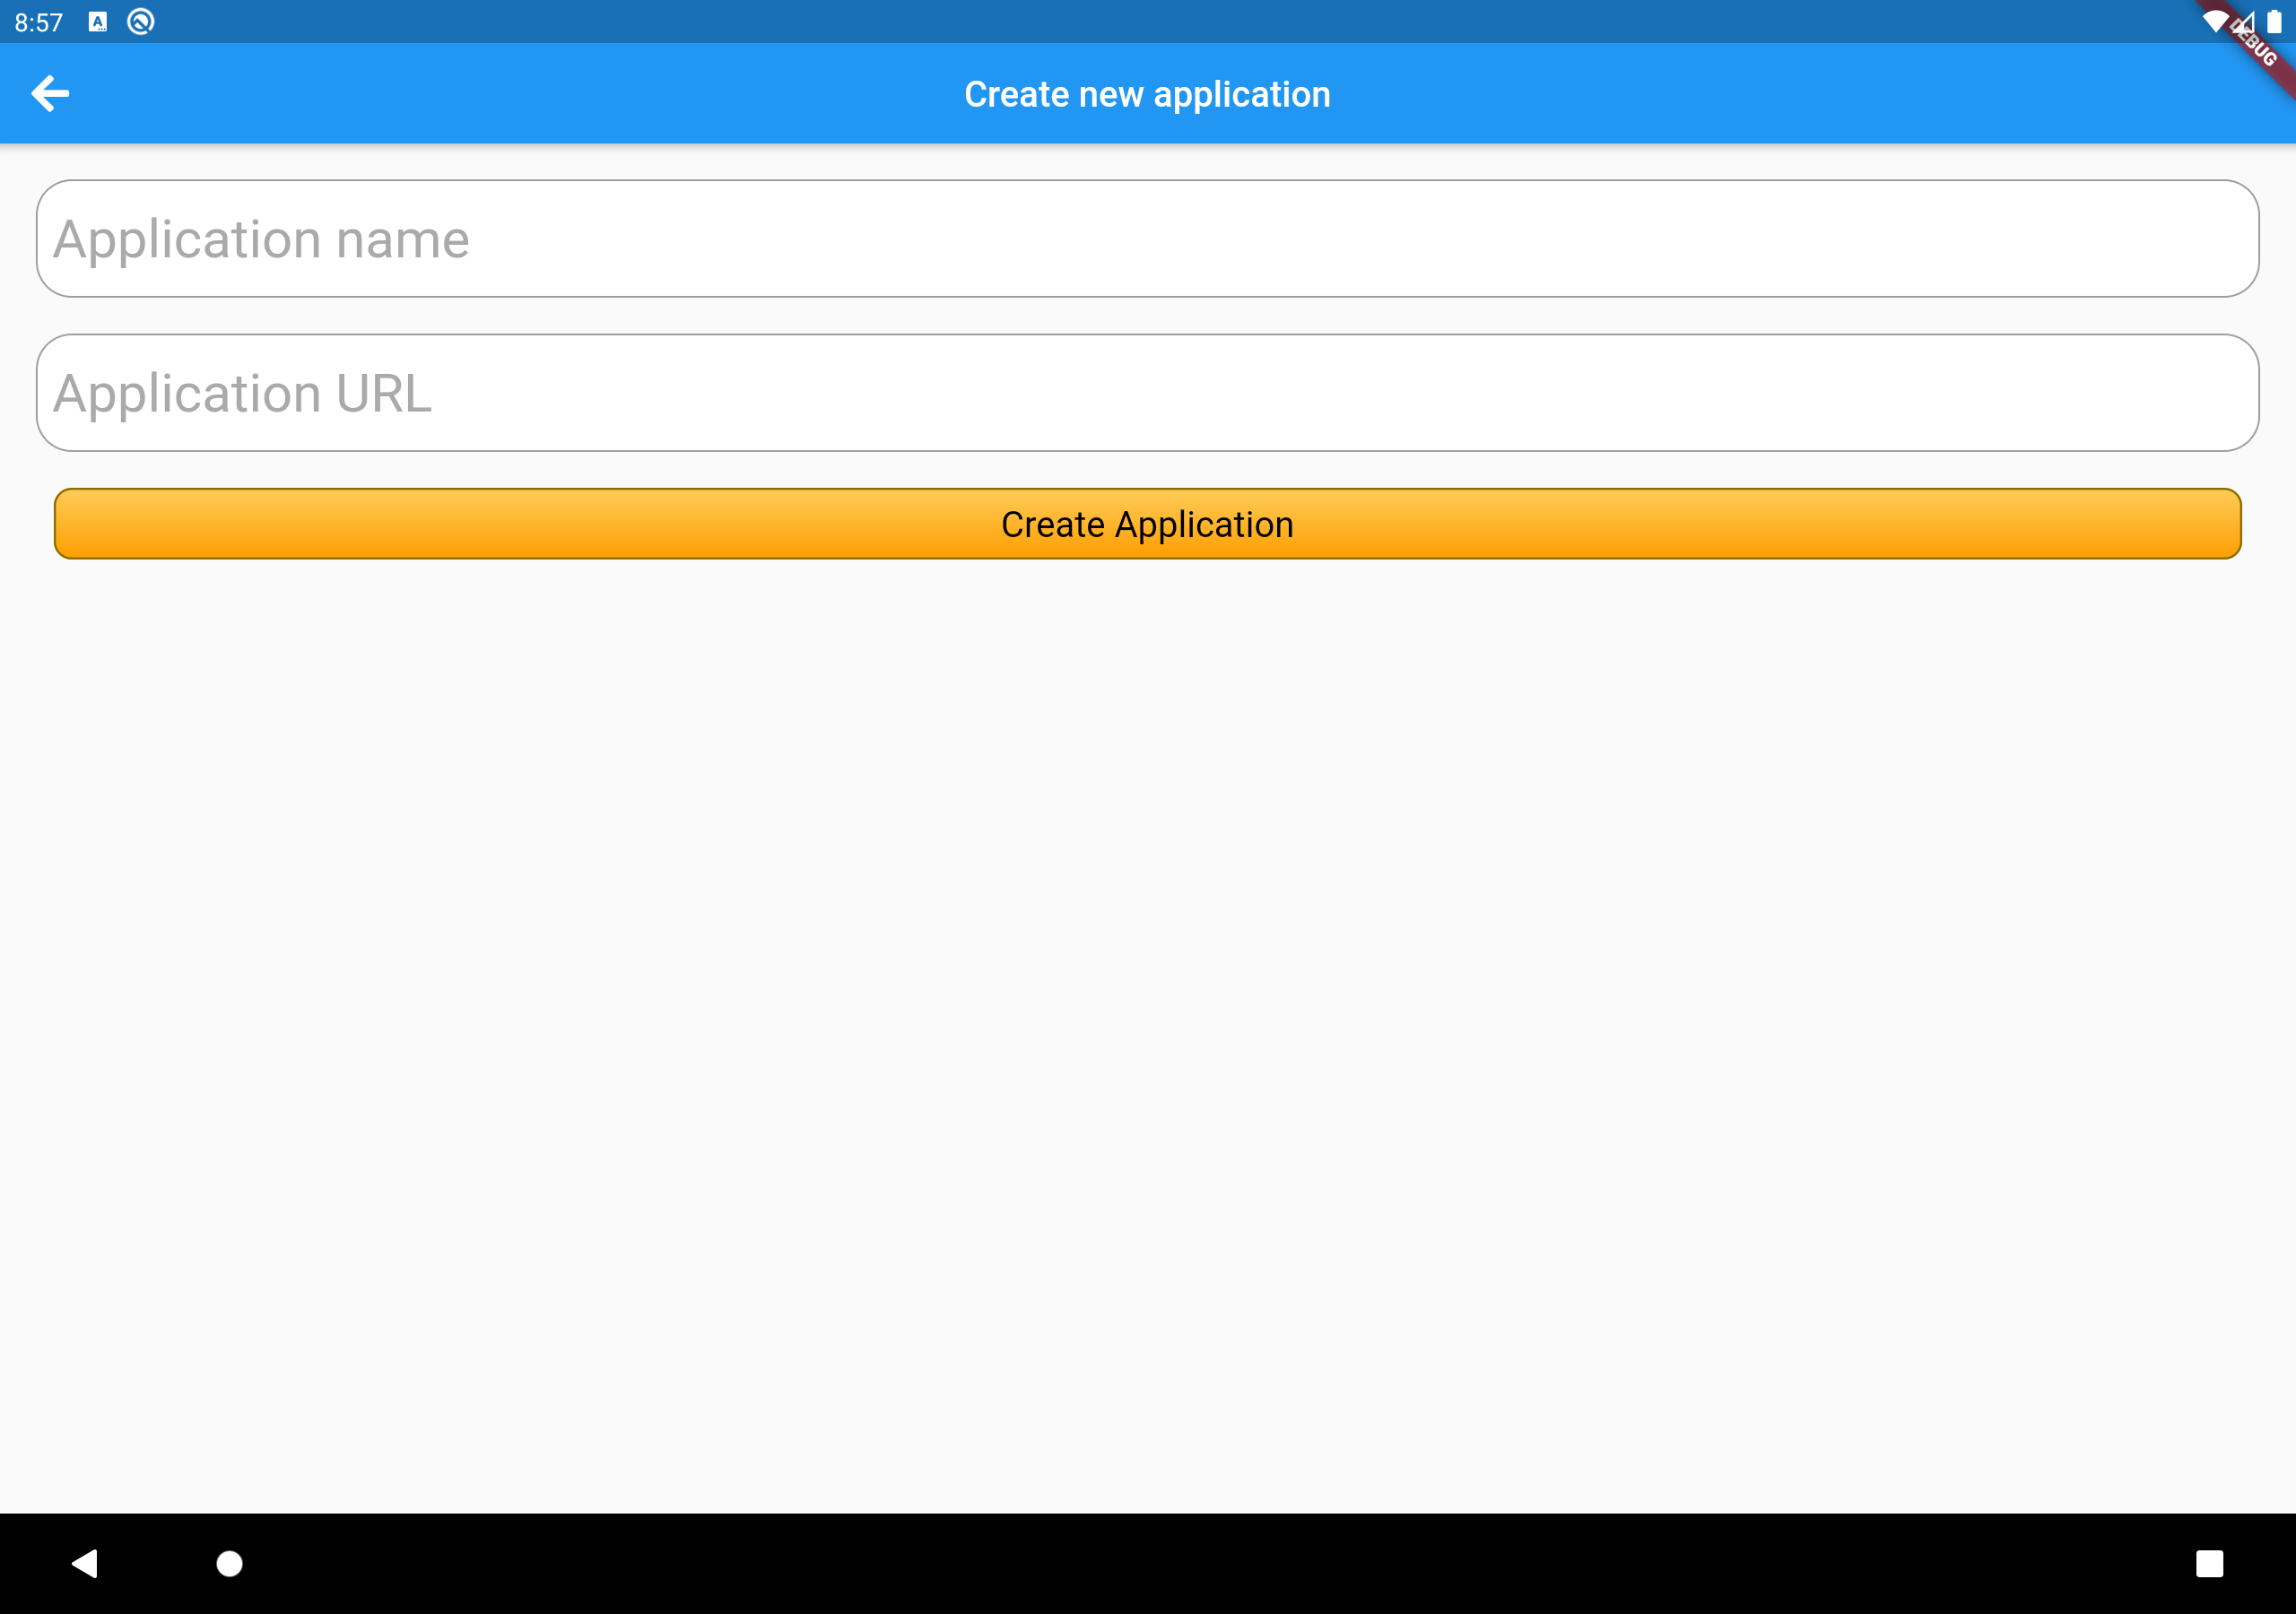
\includegraphics[width=0.9\textwidth]{Sprint_1/images/create_app_screen_app.png}
        \caption{Application creation screen implementation.}
        \label{app_creation_screen_app}
    \end{minipage}\hfill
    \begin{minipage}{0.45\textwidth}
        \centering
        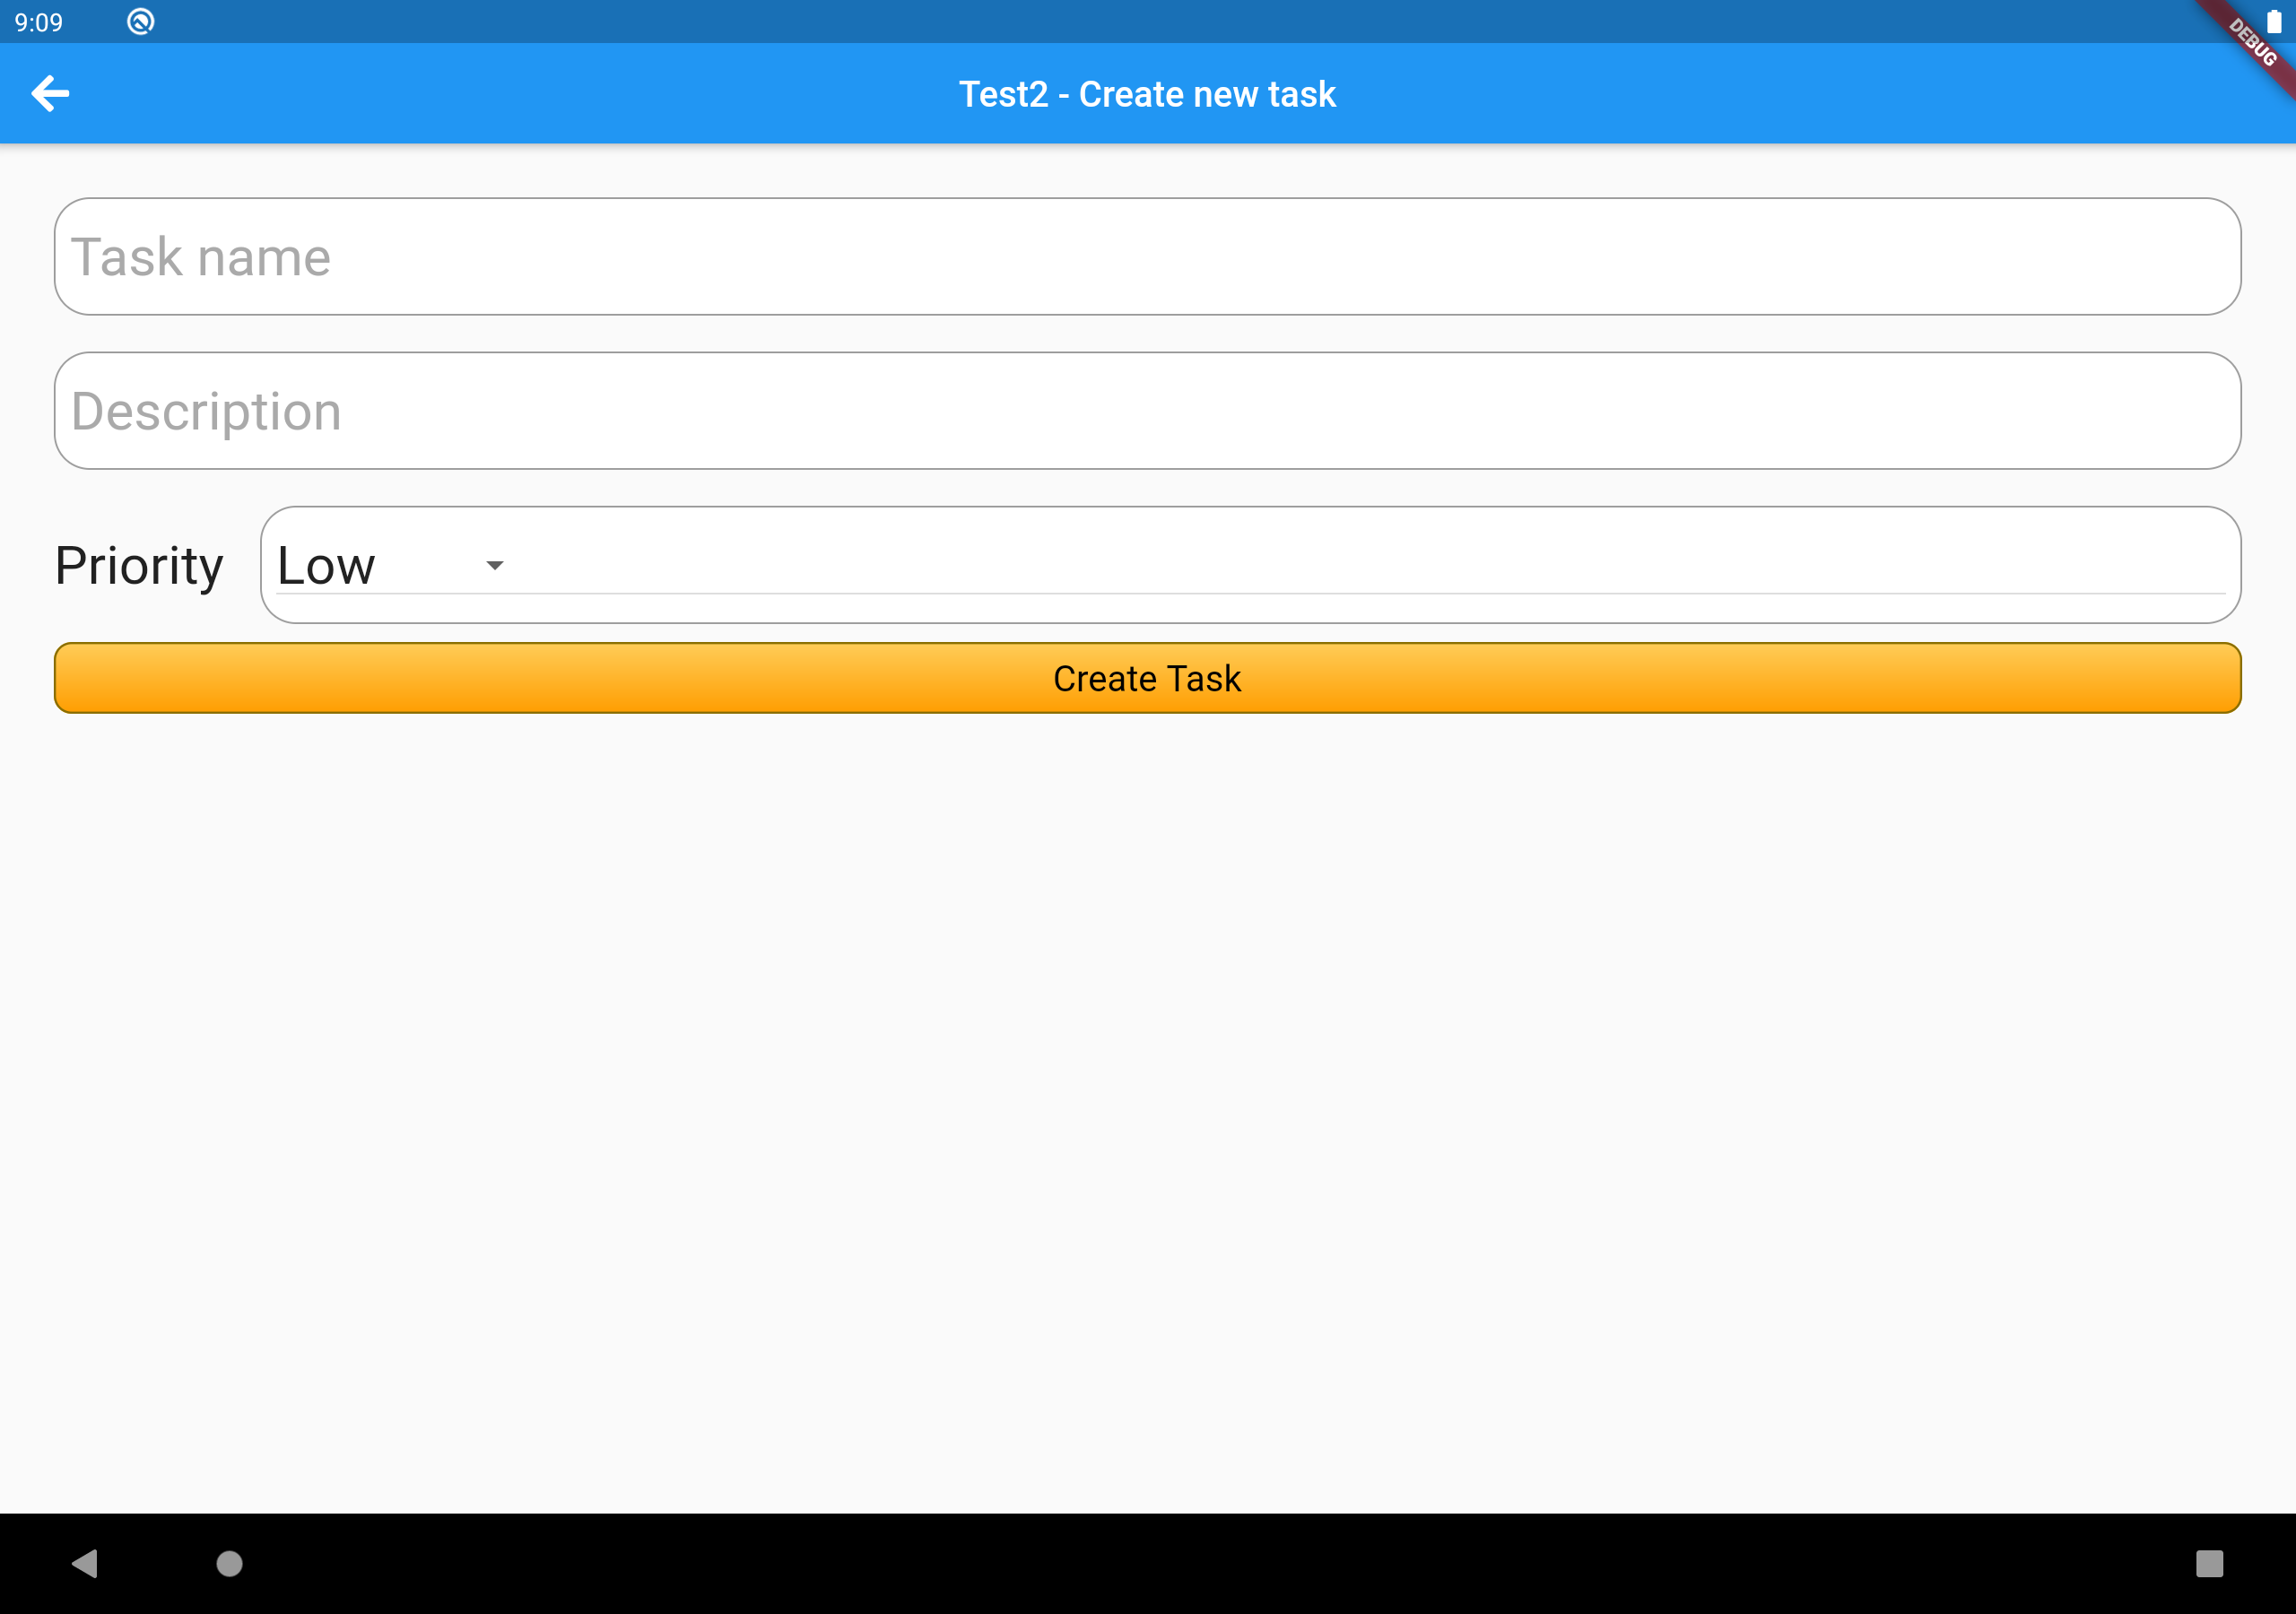
\includegraphics[width=0.9\textwidth]{Sprint_1/images/create_task_screen_app.png}
        \caption{Create task screen implementation.}
        \label{create_task_screen_app}
    \end{minipage}
\end{figure}

\begin{figure}[H]
    \centering
    \begin{minipage}{0.45\textwidth}
        \centering
        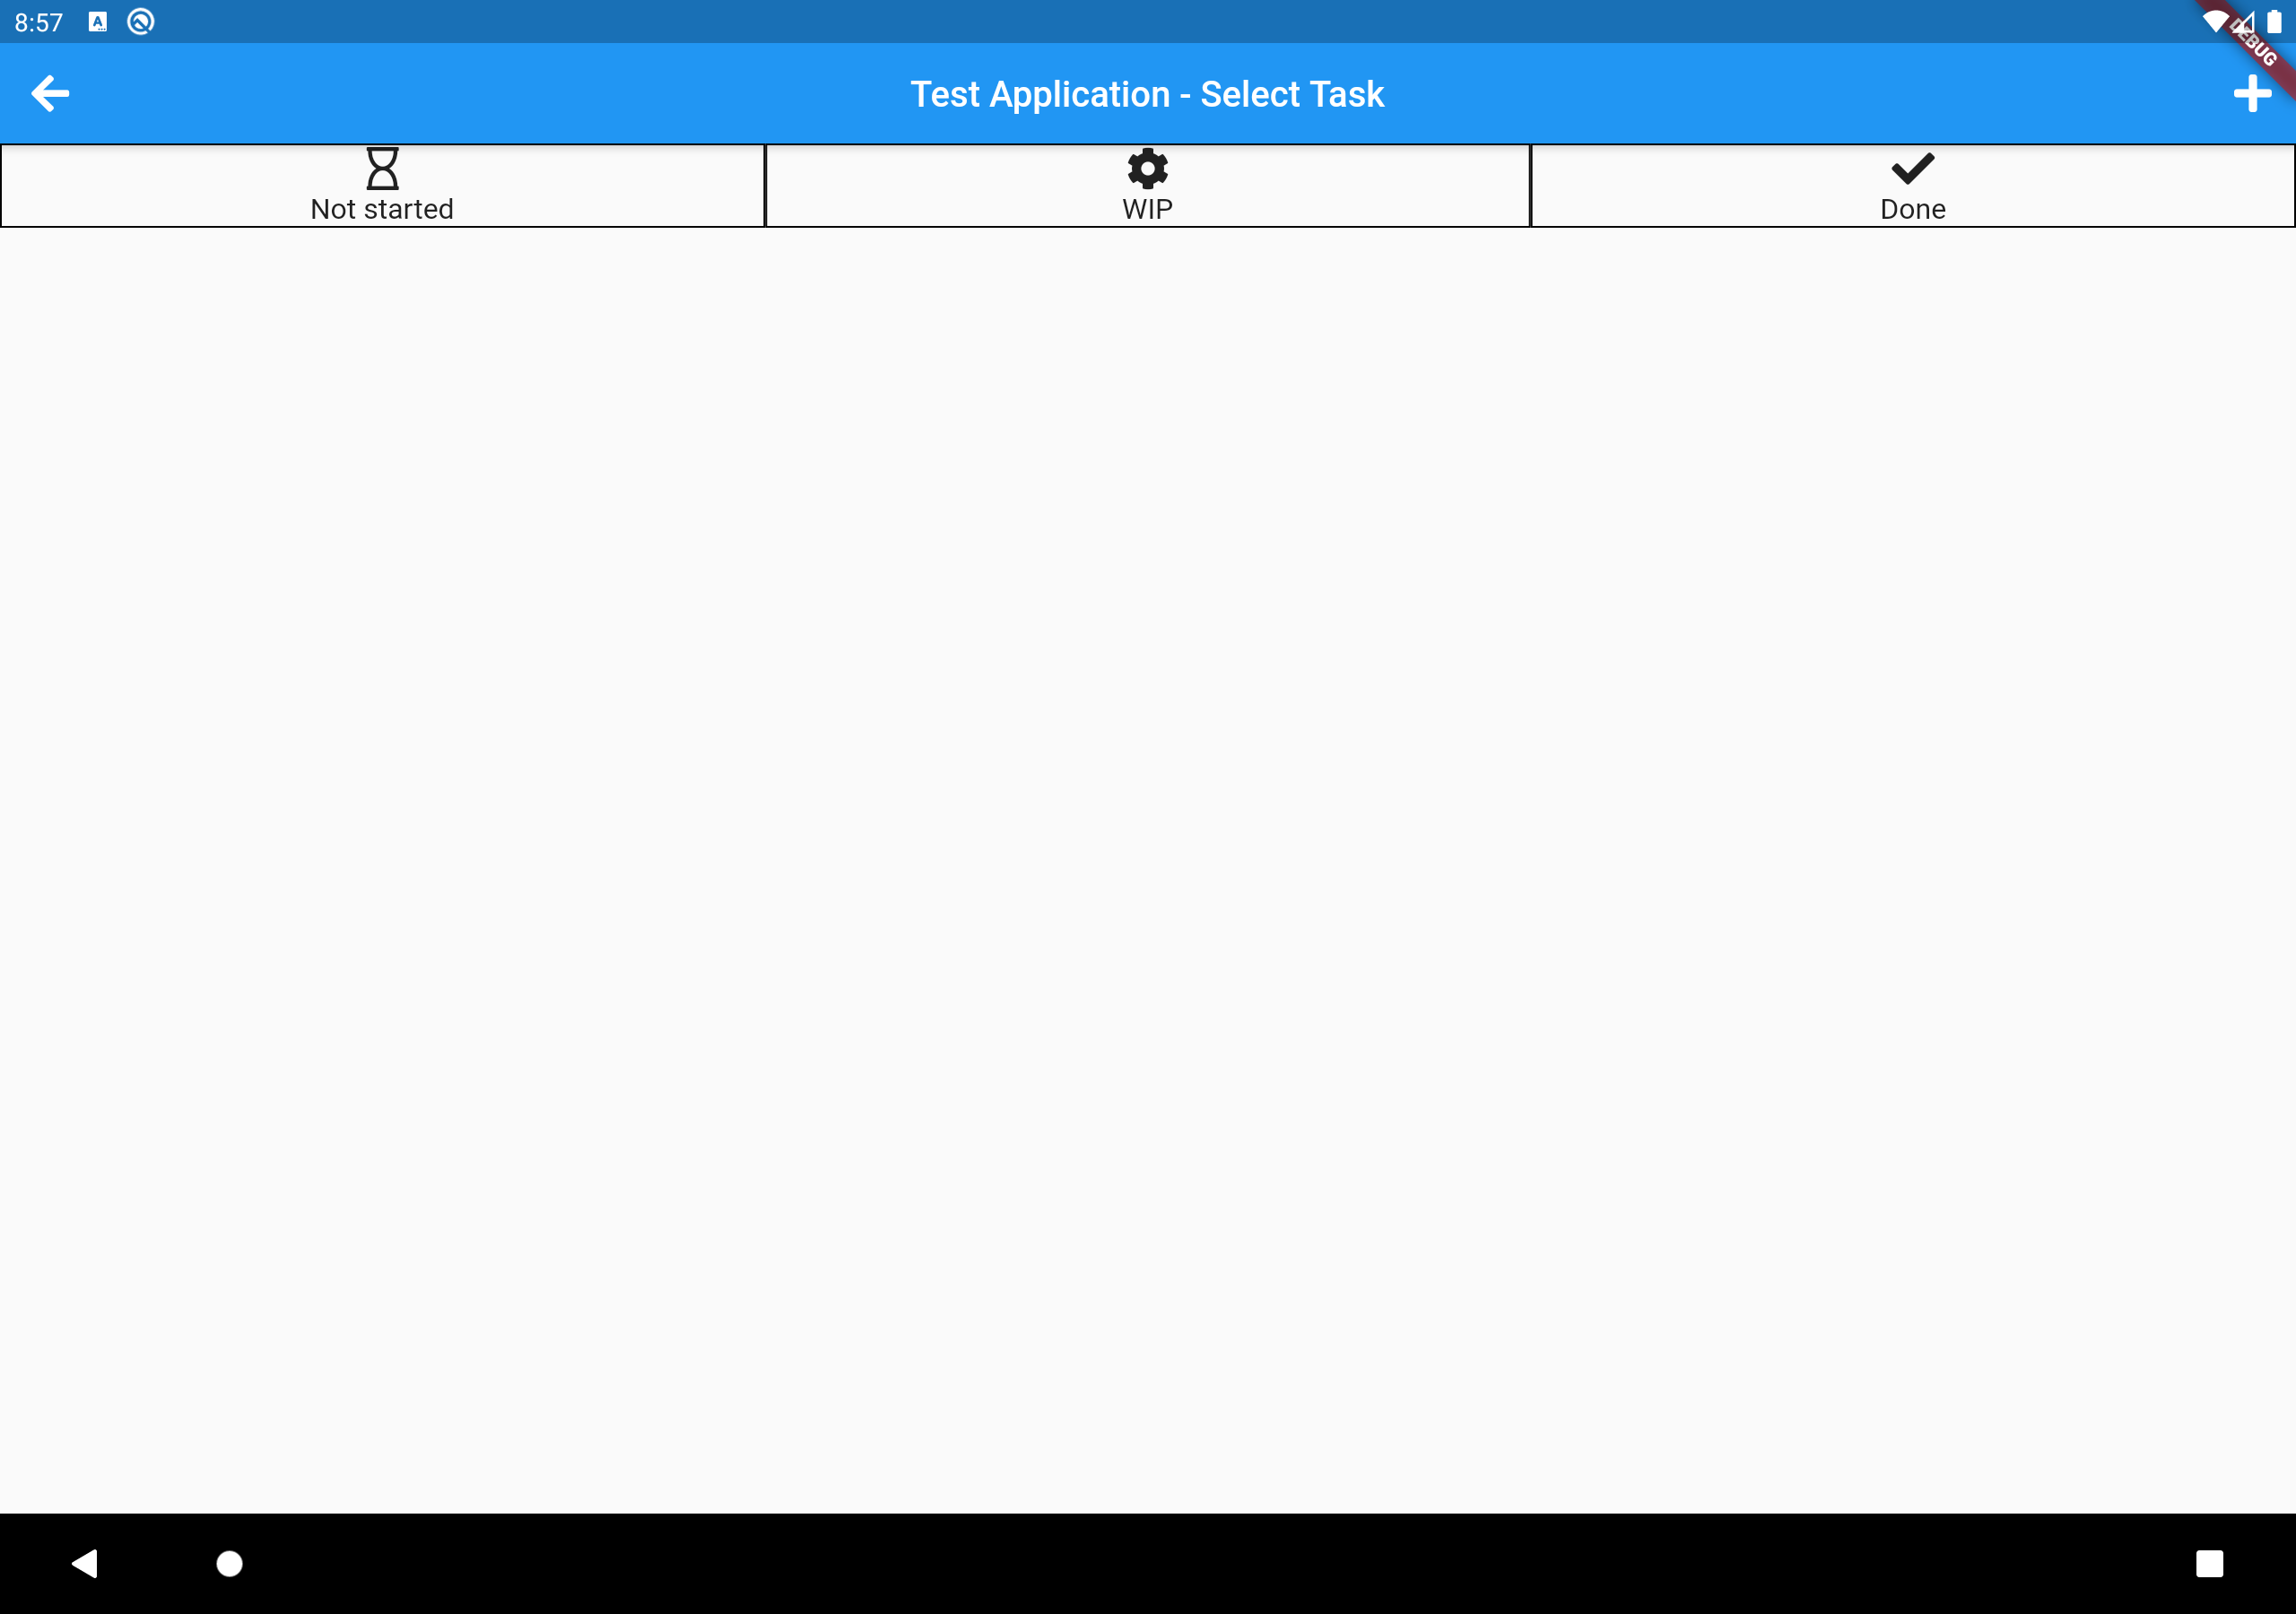
\includegraphics[width=\textwidth]{Sprint_1/images/task_dashboard_screen_app.png}
        \caption{Task dashboard screen implementation.}
        \label{task_dashboard_screen_app}
    \end{minipage}\hfill
    \begin{minipage}{0.45\textwidth}
    \end{minipage}
\end{figure}
